\documentclass[10pt]{article}
\usepackage[ngerman]{babel}
\usepackage[utf8]{inputenc}
\usepackage[T1]{fontenc}
\usepackage{graphicx}
\usepackage[export]{adjustbox}
\graphicspath{ {./images/} }
\usepackage{multirow}
\usepackage{hyperref}
\hypersetup{colorlinks=true, linkcolor=blue, filecolor=magenta, urlcolor=cyan,}
\urlstyle{same}

\title{Bachelor of Science (BSc) in Informatik Modul Software-Entwicklung 1 (SWEN1) }

\author{}
\date{}


\begin{document}
\maketitle
\section*{LE 10 - Implementation, Refactoring und Testing}
SWEN1/PM3 Team:\\
R. Ferri (feit), D. Liebhart (lieh), K. Bleisch (bles), G. Wyder (wydg)

\section*{Um was geht es?}
\begin{itemize}
  \item Wie kann ich aus den Design Artefakten einen Quellcode erstellen?
  \item Wie kann ich den Quellcode an neue Anforderungen anpassen bzw. die Qualität des Quellcodes kontinuierlich verbessern?
  \item Wie kann ich mit Hilfe von Tests die Voraussetzung für Refactoring schaffen?\\
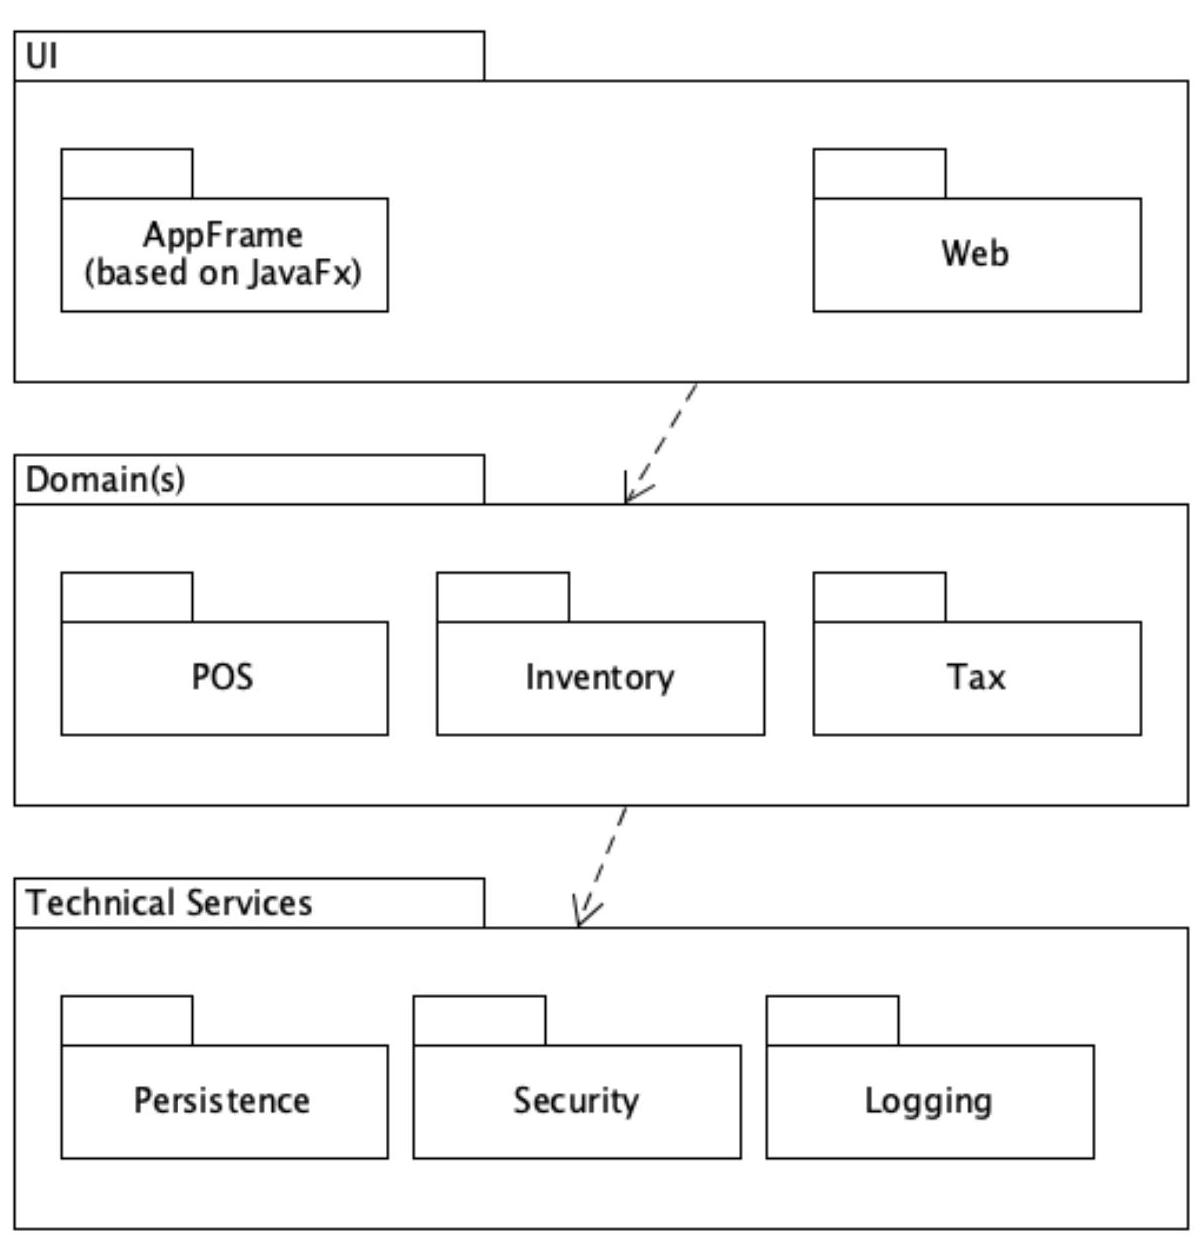
\includegraphics[width=\linewidth]{images/2025_01_02_08b621b85f305e650c0bg-02}
\end{itemize}

\section*{Lernziele LE 10 - Implementation, Refactoring und Testing}
\begin{itemize}
  \item Sie sind in der Lage:
  \item den Quellcode aus den Design Artefakten abzuleiten,
  \item Codier-Richtlinien anzuwenden und eine zusätzliche Code Dokumentation wie Javadoc zu erzeugen,
  \item eine Umsetzungsstrategie wie Test-Driven-Development (TDD) oder BehaviorDriven Devlopment (BDD) einzusetzen,
  \item den Quellcode mit Hilfe von Refactoring zu verbessern,
  \item im Entwicklungsprozess Tests durchzuführen und kennen die grundlegenden Testarten und weitere Teststufen.
\end{itemize}

\begin{enumerate}
  \item Design to Code
  \item Implementation
  \item Refactoring
  \item Testing
  \item Wrap-up und Ausblick
\end{enumerate}

\section*{Design To Code (recap)}
\begin{itemize}
  \item Aus den vorhandenen Design Artefakten soll der Quellcode abgeleitet werden.
  \item In der Praxis sind nur Teile des gesamten Quellcodes zusätzlich als Design Artefakte abgebildet.
\end{itemize}

\section*{Beispiel Fallstudie: NextGenPos (recap) \\
 DCD - Design Class Diagramm}
School of Engineering\\
InIT Institut für angewandte Informationstechnologie

\begin{itemize}
  \item Klassen
  \item Attribute
  \item Methoden
  \item Assoziation\\
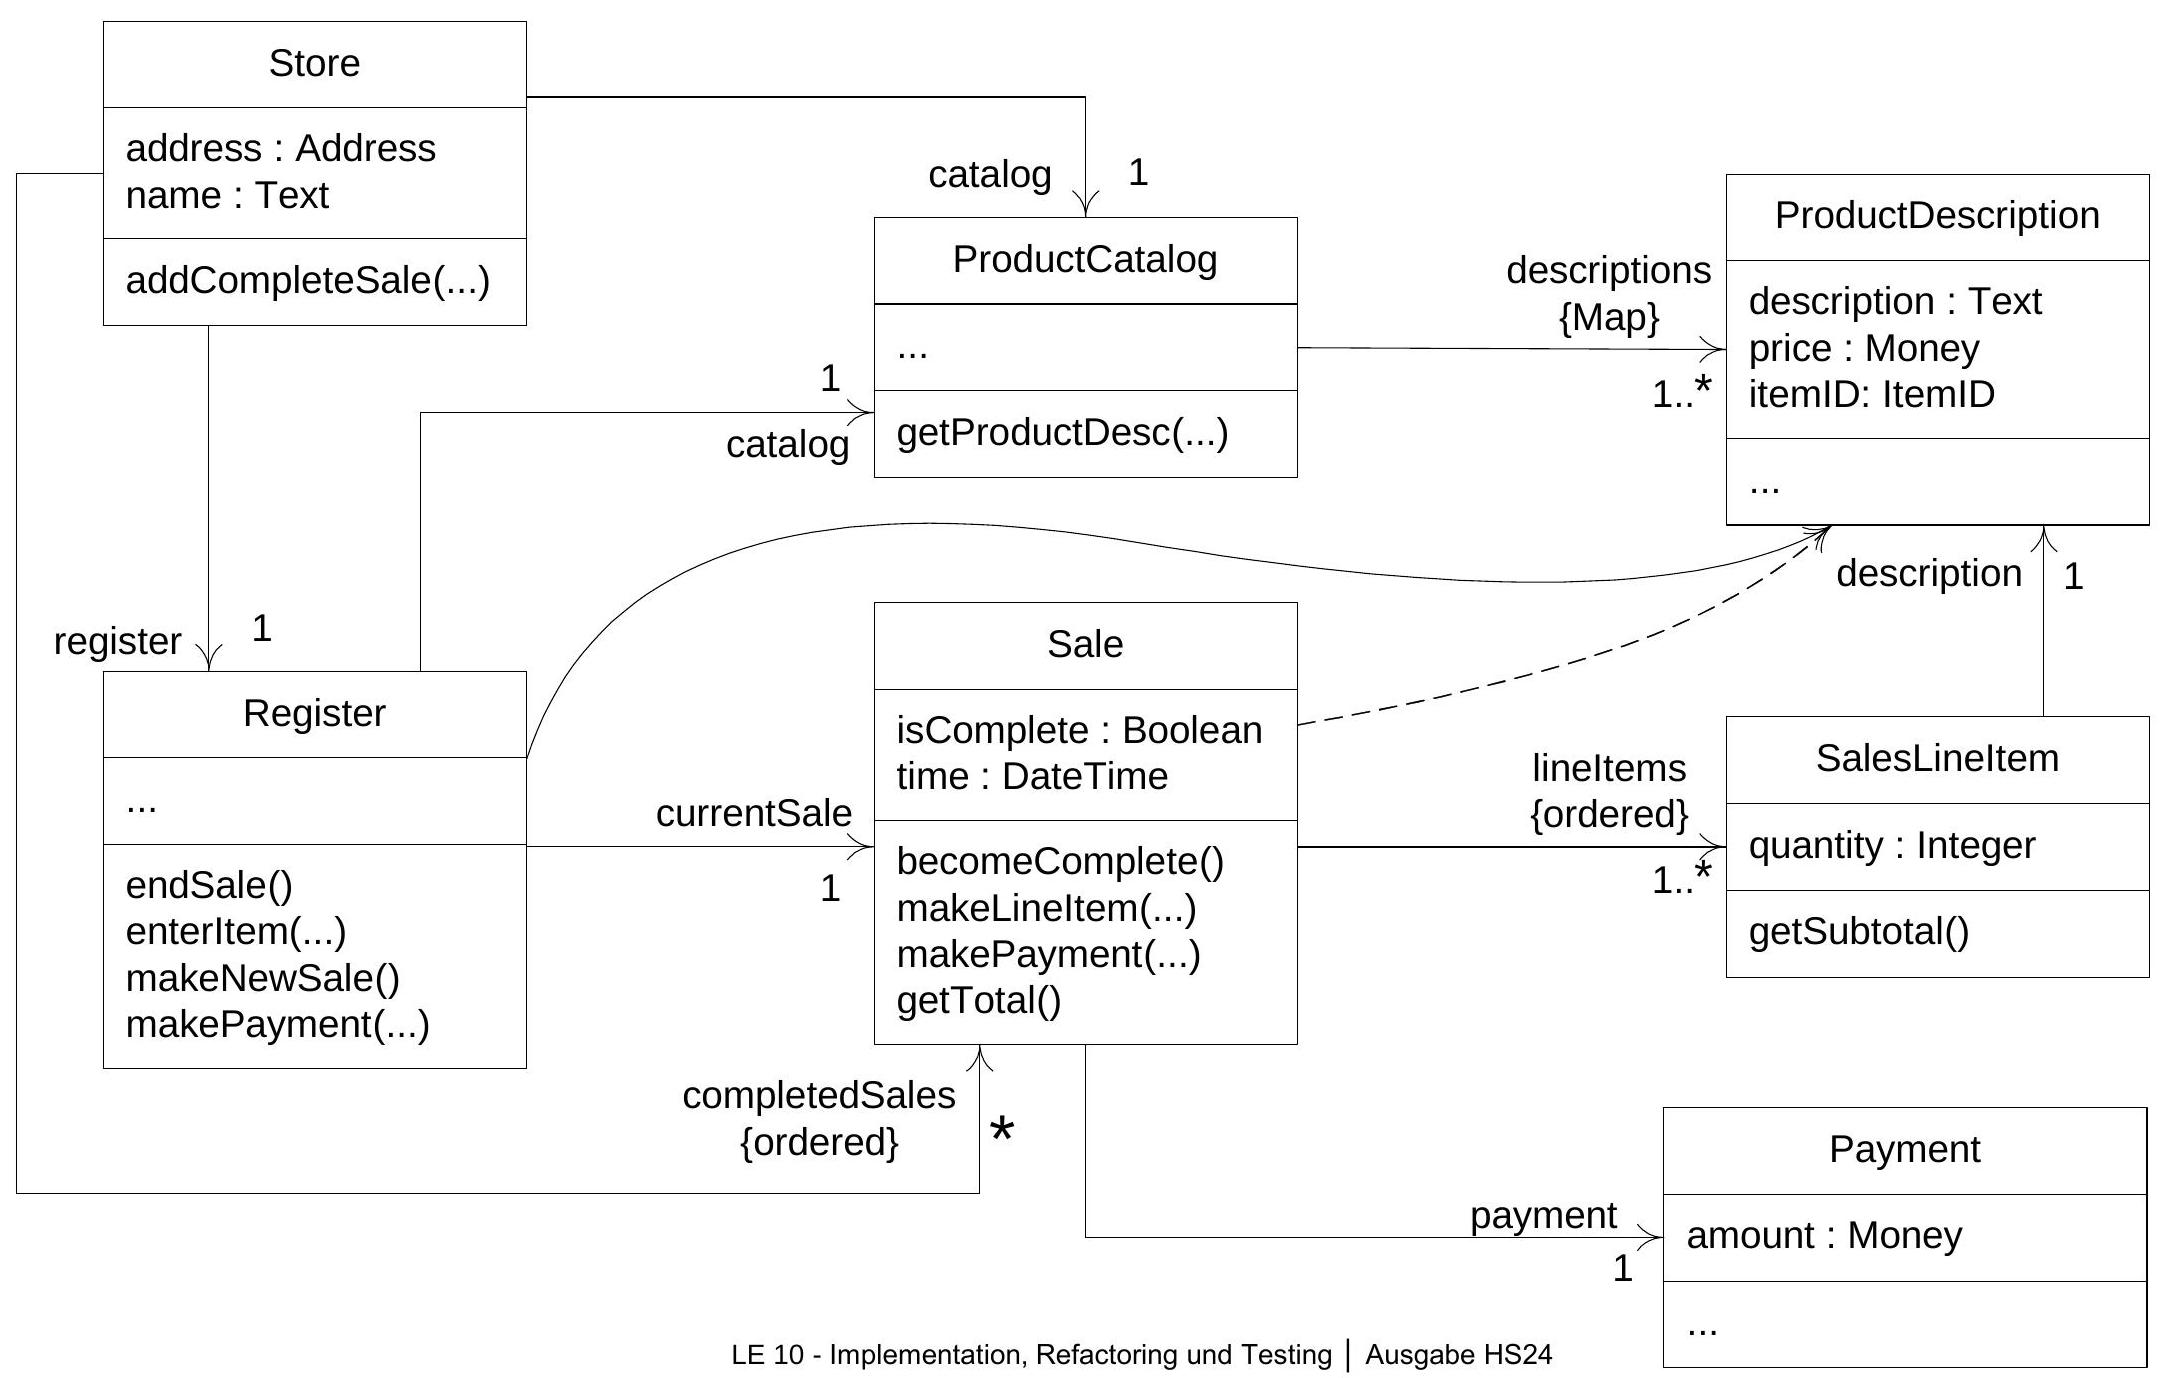
\includegraphics[width=\linewidth]{images/2025_01_02_08b621b85f305e650c0bg-06}
\end{itemize}

\section*{Beispiel Fallstudie: NextGenPos (recap) Methoden aus Interaktionsdiagrammen}
\begin{itemize}
  \item Methoden mit Signaturen\\
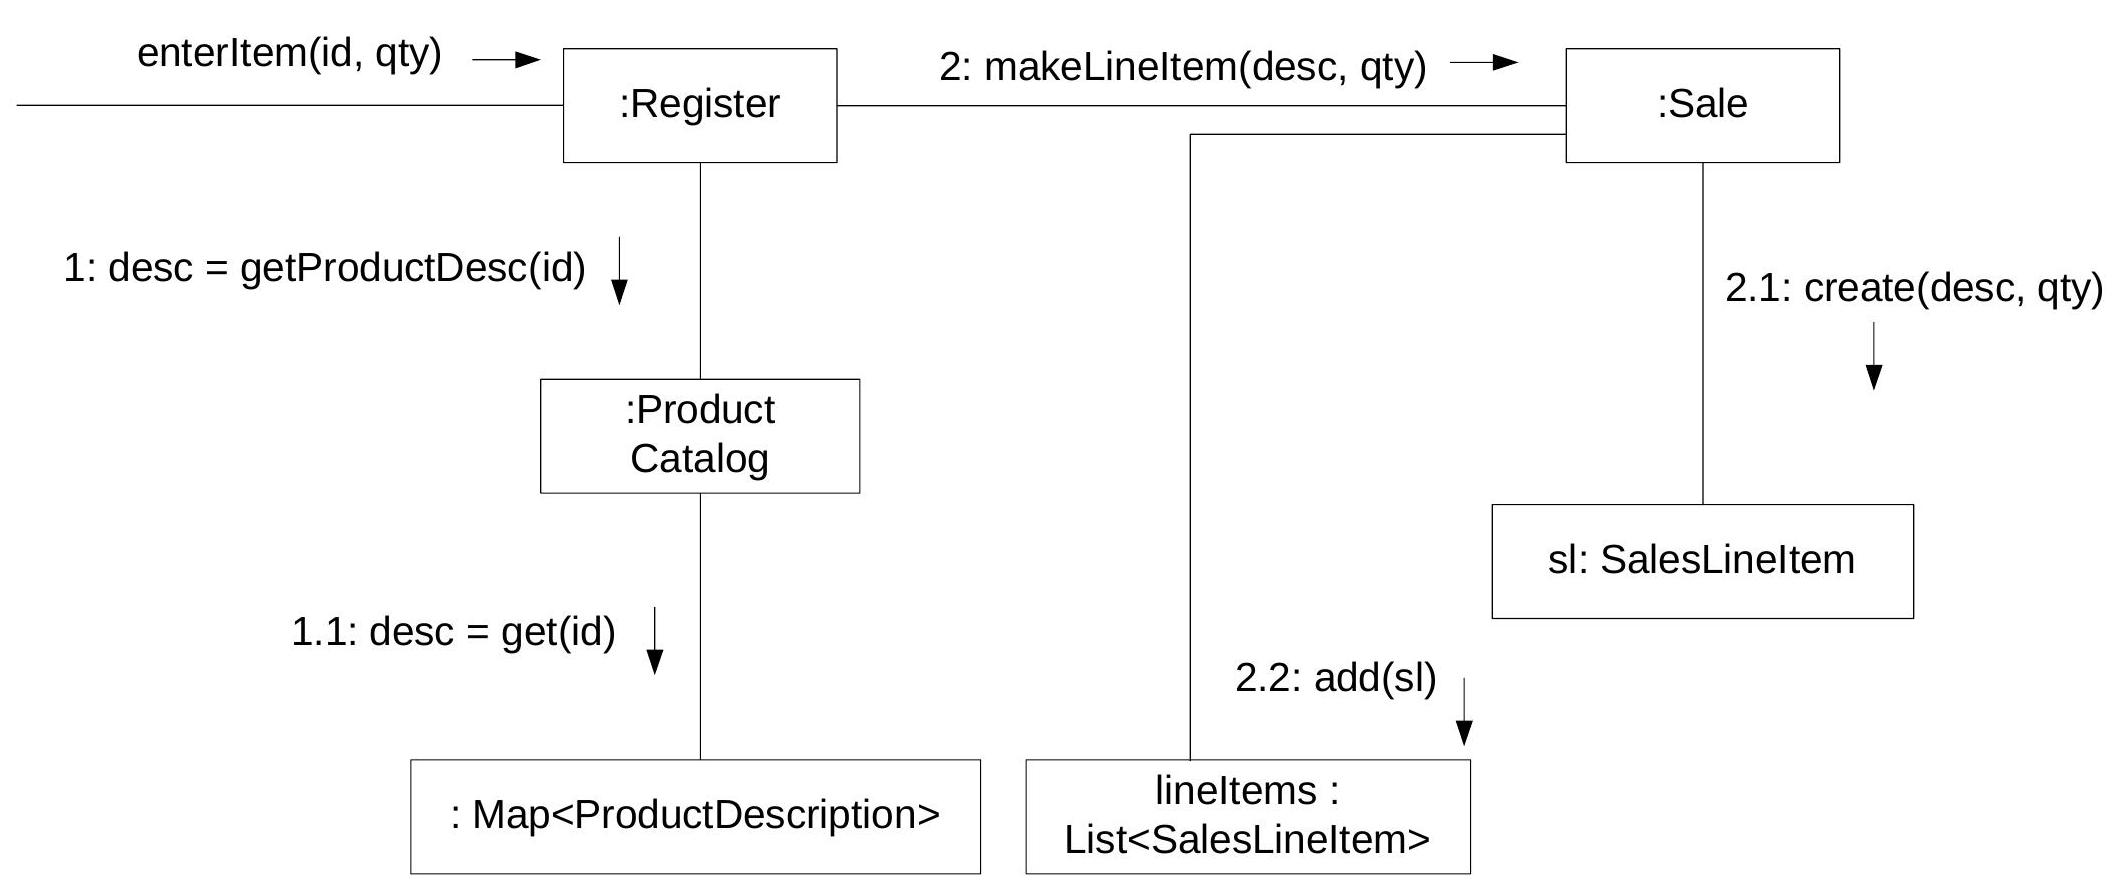
\includegraphics[width=\linewidth]{images/2025_01_02_08b621b85f305e650c0bg-07}
\end{itemize}

Register.enterItem(int itemId, int qty);\\
// Zwei Ereignisse werden an sichtbare Klassen gesendet\\
ProductDesription desc = catalog.getProductDescription(itemId); currentSale.makeLineItem(desc, qty);

\section*{Einsatz von Collection Klassen (recap)}
School of

\begin{itemize}
  \item 1 : n Beziehungen erfordern den Einsatz von Collection Klassen
  \item Die heutigen Programmiersprachen stellen ein reichhaltiges Sortiment an solchen Klassen zur Verfügung\\
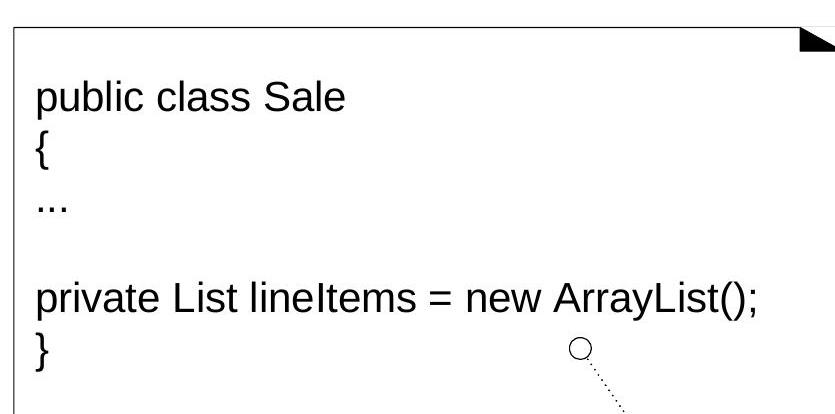
\includegraphics[width=\linewidth]{images/2025_01_02_08b621b85f305e650c0bg-08}
\end{itemize}

\begin{center}
\begin{tabular}{|c|c|c|}
\hline
Sale & \multirow[b]{3}{*}{lineltems} &  \\
\hline
isComplete : Boolean time : DateTime &  & SalesLineltem \\
\hline
becomeComplete() &  & quantity : Integer \\
\hline
\begin{tabular}{l}
makeLineltem() \\
makePayment() \\
\end{tabular} & 0 & getSubtotal() \\
\hline
\end{tabular}
\end{center}

A collection class is necessary to maintain attribute visibility to all the SalesLineltems.

Tipp: Interface und nicht Klasse deklarieren (Protected Variation!)\\
Einsatz von Generics

\section*{Fehlerbehandlung}
\begin{itemize}
  \item Exceptions verwenden.
  \item Nicht C-Style mit Errorcode als Rückgabewert
  \item Exceptions wirklich nur für Fehlersituationen verwenden, nicht für reguläre Rückgabe-Werte.
  \item Standard Exceptions verwenden.
  \item Wo sinnvoll eigene Klassen definieren.
  \item Jede Schicht kapselt Exception Handling ab und reicht diese weiter.
  \item Welche Fehlermeldungen sollen dem Benutzer angezeigt werden?
\end{itemize}

\section*{Umsetzungs-Reihenfolge: Variante Bottom-Up Strategie}
\begin{itemize}
  \item Falls alle umzusetzenden Klassen als Design Artefakte vorhanden sind, kann eine Bottom-Up Strategie gewählt werden.
\end{itemize}

Beispiel Fallstudie: NextGenPos\\
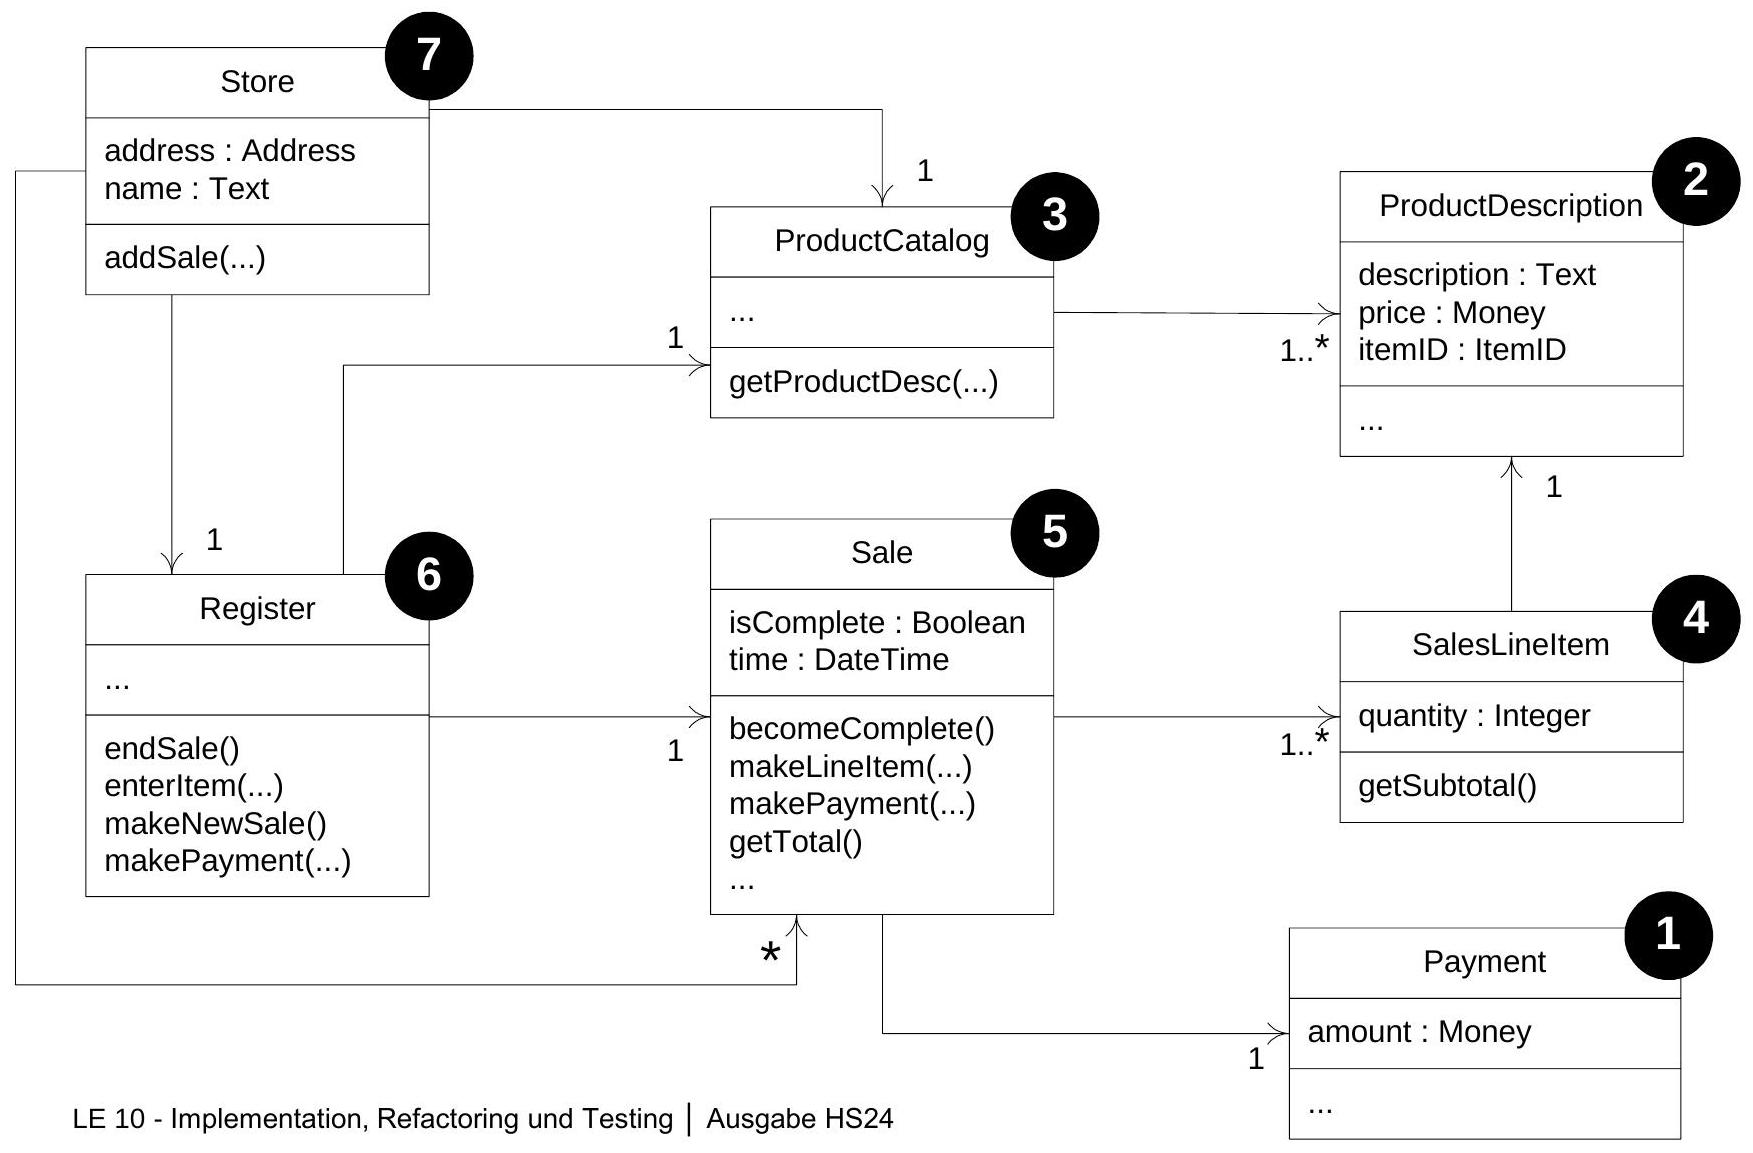
\includegraphics[width=\linewidth]{images/2025_01_02_08b621b85f305e650c0bg-10}

\section*{Umsetzungs-Reihenfolge: Variante Agile}
\begin{itemize}
  \item Im agilen Umfeld werden Funktionen Schritt für Schritt umgesetzt. Es sind nur die für die Iteration notwendigen Klassen bekannt.
  \item Vorhandene Klassen müssen angepasst (refaktoriert) werden.
  \item Die Umsetzung wird über die verschiedenen Schichten der Architektur vollzogen wie Model, Controller, Services, Repository.
  \item Ausgangspunkt ist oft eine Schnittstellenbeschreibung:
  \item Benutzerschnittstelle (von UX-Desiger)
  \item Systemschnittstelle (z.B. OpenApi Swagger)
\end{itemize}

\section*{Codierrichtlinien}
\begin{itemize}
  \item Legt verbindlich fest:
  \item Gross/Kleinschreibung
  \item Einrücken
  \item Klammernsetzung \{ \}
  \item Erleichtert Zurechtfinden in fremdem Code.
  \item Prüfprogramme für die Einhaltung der Codierrichtlinien:
  \item SonarLint
  \item Checkstyle
  \item Lint / ESLint
  \item ...
\end{itemize}

\section*{Namensgebung für Klassen, Attribute, Methoden, Variablen}
\begin{itemize}
  \item Die Namengebung ist ausserordentlich wichtig für das Codeverständnis.
  \item Unbedingt die Namensgebung der Fachdomäne im Code abbilden.
  \item Falls notwendig die deutschen Begriffe durch englische Begriffe ersetzen und in einem für alle zugänglichen Glossar beschreiben.
  \item Englische Begriffe sind zentral für den Einsatz von internationalen Entwicklern.
\end{itemize}

\begin{enumerate}
  \item Design to Code
  \item Implementation
  \item Refactoring
  \item Testing
  \item Wrap-up und Ausblick
\end{enumerate}

\section*{Implementierungsstrategie festlegen}
\begin{itemize}
  \item Code-Driven Development
  \item Zuerst die Klasse implementieren
  \item TDD: Test-Driven Development
  \item Zuerst Tests für Klassen/Komponenten schreiben, dann den Code entwickeln
  \item BDD: Behavior-Driven Development
  \item Tests aus Benutzersicht beschreiben
  \item Zum Beispiel durch die Business Analysten mit Hilfe von Gherkin
\end{itemize}

Wichtig: Unabhängig von der gewählten Implementierungsstrategie muss jedes Stück Code nach der Fertigstellung auch entsprechende Tests haben!

\section*{Erfolgsfaktoren}
\begin{itemize}
  \item Verständnis für die Aufgaben und Verantwortlichkeiten der Komponente
  \item Schnittstelle so einfach wie möglich
  \item Sinnvolle Namensgebung
  \item Code-Review Prozess durch Pull-Request's respektieren, Feedback betreffend Code-Qualität ernst nehmen
  \item Jede Programmzeile ist eine Entscheidung
\end{itemize}

\section*{Laufzeit Optimierung}
\begin{itemize}
  \item Oft wird versucht, während der Implementation, die Laufzeit zu optimieren.
  \item Sollte kritisch beobachtet werden.
  \item 3 Regeln der Optimierung:
  \item Optimiere nicht
  \item Optimiere NOCH nicht
  \item Vor der Optimierung analysieren, wo wirklich Zeit verbraucht wird
\end{itemize}

\section*{Optimierungsregeln}
\begin{itemize}
  \item Performance Monitor einsetzen.
  \item wo wird wirklich viel Zeit verbraucht !?
  \item Zeitfresser: Datenbankzugriffe pro Objekt über eine Liste
  \item Die Algorithmen optimieren.
  \item Collections.sort(...) in Java 7 ist doppelt so schnell wie der von Java 6 (!)
  \item Erst in zweiter Linie den Code anschauen
  \item Heutige Compiler optimieren bereits viel
  \item Berechnungen aus der for Schleife herausnehmen
  \item Java VM optimiert selber, und geht über «Just In Time Compilation» hinaus.
\end{itemize}

\begin{enumerate}
  \item Design to Code
  \item Implementation
  \item Refactoring
  \item Testing
  \item Wrap-up und Ausblick
\end{enumerate}

\section*{Refactoring}
\begin{itemize}
  \item Strukturierte, disziplinierte Methode, vorhandenen Code umzuschreiben
  \item Externes Verhalten bleibt gleich!
  \item Viele kleine Schritte (Codeänderungen)
  \item Interne Struktur wird verbessert.
  \item Um Erweiterungen einzuleiten
  \item Trennen von der eigentlichen Weiterentwicklung!
  \item Low Level Design - Programmiertechnik
\end{itemize}

\section*{Code verbessern ...}
\begin{itemize}
  \item DRY: Keinen duplizierten Code
  \item Namensgebung: Klarheit erhöhen, Aussagekräftige Namen
  \item Lange Methoden verkürzen (kein Spaghetti-Code -> neue Methoden)
  \item Algorithmen strukturieren in
  \item Initialisierung
  \item Berechnung
  \item Aufbereiten des Resultats
  \item Sichtbarkeit verbessern
  \item Testbarkeit verbessern
\end{itemize}

\section*{Was sind Code Smells?}
\begin{itemize}
  \item Duplizierter Code
  \item Lange Methoden
  \item Klassen mit vielen Instanzvariablen
  \item Klassen mit sehr viel Code
  \item Auffällig ähnliche Unterklassen
  \item Keine Interfaces, nur Klassen
  \item Hohe Kopplung zwischen Klassen
\end{itemize}

\section*{Unterstützung durch ...}
\begin{itemize}
  \item Automatisierte Tests
  \item Stellen sicher, dass nach dem Refactoring der Code immer noch funktioniert
  \item Moderne Entwicklungsumgebungen
  \item Automatisieren alle abhängigen Arbeitsschritte
  \item Beispiel: Nach einer Umbenennung einer Variablen werden alle Verwendungen dieser Variablen ebenfalls geändert
\end{itemize}

\section*{Refactoring Patterns (1/2)}
\begin{itemize}
  \item \href{http://www.refactoring.com}{www.refactoring.com}
  \item Rename Method / Class / Variable
  \item Eine Methode/Klasse/Variable wird so umbenannt, dass sie einen aussagekräftigen Namen erhält.
  \item Pull Up / Push Down
  \item Eine Methode wird in eine Superklasse / Subklasse verschoben.
  \item Extract Interface / Superclass
  \item Ein Teil eines bestehenden Interfaces / Klasse wird in eine Superinterface / Superklasse extrahiert.
\end{itemize}

\section*{Refactoring Patterns (2/2)}
\begin{itemize}
  \item Extract Method
  \item Teil einer Methode in eine private Methode auslagern.
  \item Extract Constant
  \item Symbolische Konstante verwenden.
  \item Introduce Explaining Variable
  \item Grossen Ausdruck aufteilen, erklärende Zwischenvariablen einfügen.
\end{itemize}

\section*{Methode extrahieren - kein Spaghetti-Code}
\begin{verbatim}
public void takeTurn(){
    // roll dice
    int rollTotal = 0;
    for (int i = 0; i < dice.length; i++){
        dice[i].roll();
        rollTotal += dice[i].getFaceValue();
    }
    Square newLoc=board.getSquare(
    piece.getLocation(), rollTotal);
    piece.setLocation(newLoc);
}
\end{verbatim}

Lange Codefragmente mit Kommentaren wie //roll dice\\
mit verständlichen Methoden verkleinern

\begin{verbatim}
public void takeTurn(){
    // the refactored helper method
        int rollTotal = rollDice();
        Square newLoc = board.getSquare(
            piece.getLocation(), rollTotal);
        piece.setLocation(newLoc);
}
private int rollDice(){
    int rollTotal = 0;
    for (int i = 0; i < dice.length; i++){
        dice[i].roll();
        rollTotal += dice[i].getFaceValue();
    }
    return rollTotal;
}
\end{verbatim}

\begin{enumerate}
  \item Design to Code
  \item Implementation
  \item Refactoring
  \item Testing
  \item Wrap-up und Ausblick
\end{enumerate}

\section*{Denkpause}
\section*{Aufgabe 7.6 (3’)}
\section*{Fragen:}
\begin{itemize}
  \item Sie sollen für die Klasse Sale einen Unit-Test schreiben (Design-Klassendiagramm folgt auf der nächsten Folie).
  \item Was ist dabei das Problem für einen reinen Unit-Test?
  \item Wie kann es gelöst werden?
\end{itemize}

\section*{Denkpause}
School of\\
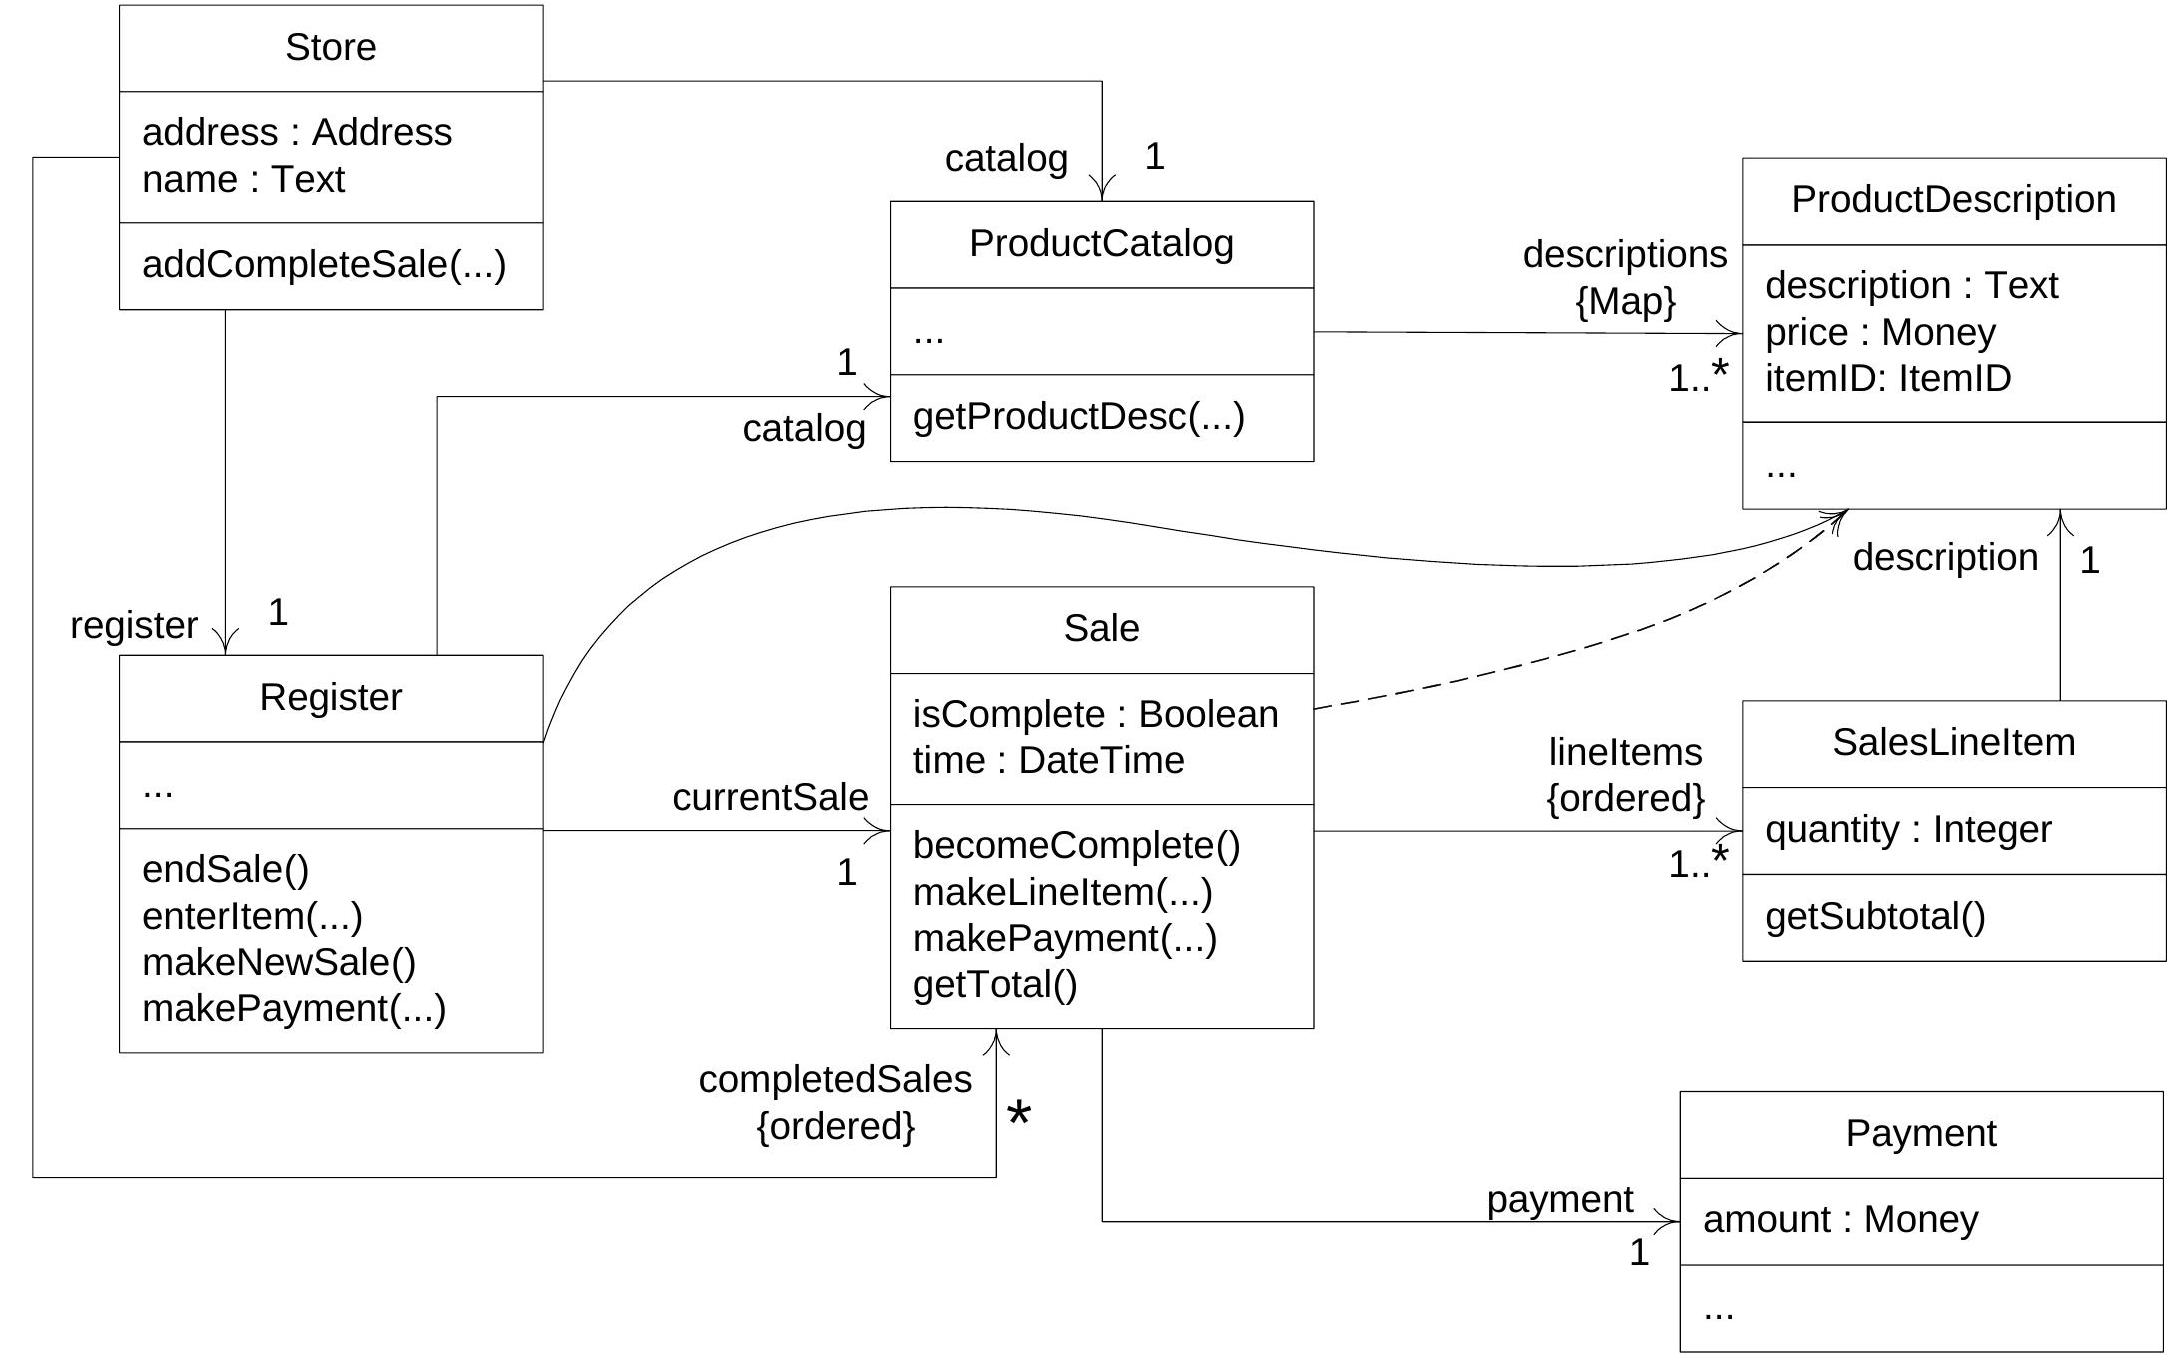
\includegraphics[width=\linewidth]{images/2025_01_02_08b621b85f305e650c0bg-29}

\section*{Repetition Grundlegende Testarten}
\begin{itemize}
  \item Funktionaler Test (Black-Box Verfahren)
  \item Nicht funktionaler Test (Lasttest etc.)
  \item Strukturbezogener Test (White-Box Verfahren)
  \item Änderungsbezogener Test (Regressionstest etc.)
\end{itemize}

\section*{Weitere Teststufen und Testarten}
\begin{itemize}
  \item Integrationstest
  \item Systemtest
  \item Abnahmetest
  \item Regressionstest
\end{itemize}

\section*{Wichtige Begriffe}
\begin{itemize}
  \item Testling, Testobjekt
  \item Objekt, das getestet wird
  \item Fehler
  \item Der Entwickler macht einen Fehler
  \item Fehlerwirkung, Bug
  \item Jedes zu den Spezifikationen abweichende Verhalten
  \item Testfall
  \item Satz von Testdaten zur vollständigen Ausführung eines Tests
  \item Testtreiber
  \item Rahmenprogramm, das den Test startet und ausführt
\end{itemize}

\section*{Merkmale (1/2)}
School of

\begin{itemize}
  \item Was wird getestet?
  \item Eine Einheit / Klasse (Unit-Test)
  \item Zusammenarbeit mehrerer Klassen
  \item Die gesamte Applikationslogik (ohne UI)
  \item Die gesamte Anwendung (über UI)
  \item Wie wird getestet?
  \item Dynamisch: Testfall wird ausgeführt
  \item Black-Box Test
  \item White-Box Test
  \item Statisch: Quelltext wird analysiert
  \item Walkthrough, Review, Inspektion
\end{itemize}

\section*{Merkmale (2/2)}
School of

\begin{itemize}
  \item Wann wird der Test geschrieben?
  \item Vor dem Implementieren (Test-Driven Development, TDD)
  \item Nach dem Implementieren
  \item Wer testet?
  \item Entwickler
  \item Tester, Qualitätssicherungsabteilung
  \item Kunde, Endbenutzer
\end{itemize}

\begin{enumerate}
  \item Design to Code
  \item Implementation
  \item Refactoring
  \item Testing
  \item Wrap-up und Ausblick
\end{enumerate}

\begin{itemize}
  \item Die Umsetzung des Entwurfs in Code ist eine anspruchsvolle Aufgabe und braucht Disziplin.
  \item Es muss von Anfang an eine Umsetzungsstrategie wie z.B. TDD gewählt werden.
  \item Refactoring ist im agilen Umfeld eine zentrale Tätigkeit. Sie dient der kontinuierlichen Qualitätsverbesserung.
  \item Testing ist die Voraussetzung für Refactoring.
  \item Ohne eine genügende Testabdeckung ist Refactoring sehr risikobehaftet und bewirkt ein fehleranfälliges Software-Produkt.
\end{itemize}

\section*{Ausblick}
\begin{itemize}
  \item In den nächsten drei Lerneinheiten werden wir:
  \item je ein Thema vertiefen (3 aus 4).
  \item Verteilte System
  \item GUI-Architekturen
  \item Persistenz
  \item Framework-Design
\end{itemize}

\section*{Quellenverzeichnis}
[1] Spillner, A. und Linz, T.: Basiswissen Softwaretest, dpunkt-Verlag, 2019\\[0pt]
[2] Fowler, M.: Refactoring, Addison-Wesley, 2018\\[0pt]
[3] Fowler, M.: Test Driven Design, Addison-Wesley, 2005


\end{document}